\section{实验}

\subsection{数据集和指标}
我们使用YCB-V数据集\cite{xiang2018posecnn}和IC-BIN数据集\cite{icbin}验证我们的方法,遵循BOP挑战赛\cite{hodan2024bop}的设置和指标。我们的方法利用50,000张合成图像进行训练,并在真实图像上进行测试。评估基于三个指标:可见表面差异(VSD)、最大对称感知表面距离(MSSD)和最大对称感知投影距离(MSPD)。这三个指标的平均值,记为AR,作为整体性能指标。

\subsection{与现有技术的比较}
\begin{table}[ht]
        \centering
        \caption{
                YCB-V数据集上的BOP评估结果
        }
        \resizebox{\textwidth}{!}{%
        \begin{tabular}{l c c c c c c c c}
        \toprule
        6D 物体位姿估计方法 & 输入类型 & 训练类型&$AR\uparrow$&$AR_{VSD}\uparrow$&$AR_{MSSD}\uparrow$&$AR_{MSPD}\uparrow$&时间(s)$\downarrow$\\       %表格第一行,&的位置对齐
        \midrule
        CDPNv2~\cite{li2019cdpn}&RGB&PBR&53.2&39.6&57.0&63.1&0.143 \\
        CosyPose~\cite{labbe2020cosypose}&RGB&PBR&57.4&51.6&55.4&65.3&0.342\\
        EPOS~\cite{hodan2020epos}&RGB&PBR&49.9&41.1&46.4&62.1&0.764 \\
        SurfEmb~\cite{haugaard2022surfemb}&RGB&PBR&64.7&54.8&62.0&77.3&5.427 \\
        GDRNPP~\cite{wang2021gdr}&RGB&PBR&71.3&59.9&70.8&\textbf{83.1}&0.277\\
        ZebraPoseSAT-EffnetB4~\cite{su2022zebrapose}&RGB&PBR&72.9&64.0&72.5&82.1&0.25 \\
        SymNet~\cite{symnet}&RGB&PBR&73.9&63.8&75.1&82.6&\textbf{0.091} \\
        Contour Alignment(本章)&RGB&PBR&\textbf{74.8}&\textbf{66.0}&\textbf{75.3}&\textbf{83.1}&0.110\\
        \midrule
        CDPNv2+ICP~\cite{li2019cdpn}&RGB-D&PBR+real&61.9&59.0&70.1&56.5&0.637\\
        Pix2Pose+ICP~\cite{park2019pix2pose}&RG-D&PBR+real&67.5&69.3&70.3&63.0&2.106\\
        \midrule
        FFB6D~\cite{he2021ffb6d}&RGB-D&PBR&75.1&70.6&82.7&74.0&0.199\\
        \bottomrule
        \end{tabular}
        }
\label{tab:ca_ycbv_bop}
\end{table}

\begin{table}[htbp]
        \centering
        \caption{
                IC-BIN 数据集上的 BOP 评估结果
        }
        \resizebox{\textwidth}{!}{%
        \begin{tabular}{l c c c c c c c c}
        \toprule
        6D 物体位姿估计方法 &输入类型&训练类型&$AR\uparrow$&$AR_{VSD}\uparrow$&$AR_{MSSD}\uparrow$&$AR_{MSPD}\uparrow$&时间 (s)$\downarrow$\\
        \midrule
        CRT-6D~\cite{castro2023crt}&RGB&pbr&53.7&\textbf{47.7}&51.7&61.8&0.120 \\
        ZebraPoseSAT-EffnetB4&RGB&pbr&54.5&47.5&\textbf{53.5}&62.5&0.25 \\
        SymNet&RGB&pbr&\textbf{54.7}&45.0&51.1&\textbf{67.8}&\textbf{0.088} \\
        Contour Alignment(本章)&RGB&pbr&\textbf{54.7}&45.4&51.1&67.7&0.098 \\
        \bottomrule
        \end{tabular}
        }
\label{tab:ca_icbin_bop}
\end{table}
我们将我们的结果与完全在合成数据上训练的其他方法进行比较,特别是在YCB-V数据集和IC-BIN数据集上,如\autoref{tab:ycbv_bop}和\autoref{tab:icbin_bop}所示。术语“PBR”表示模型完全在合成图像上训练,而“RGB”表示输入中未使用深度信息。向上箭头(↑)表示较高的指标值表示更好的性能,而向下箭头(↓)表示相反。我们采用BOP挑战赛2023\cite{hodan2024bop}提供的默认检测结果。与其他方法相比,我们的方法运行时间显著减少,因为我们的细化方法不依赖于另一个耗时的网络。我们的方法在准确性和运行时间方面都取得了优异的结果。具体来说,我们比基线模型SymNet\cite{symnet}提高了$0.9\%$,并且在不使用深度信息的情况下,达到了接近使用RGB-D图像作为输入的FFB6D\cite{he2021ffb6d}的准确性。

\subsection{消融研究}

我们进行了深入的消融研究,以研究各种因素对我们方法的影响,包括Tikhonov正则化、早停和迭代次数。所有消融研究均在YCB-V数据集上进行,使用平均召回率(AR)作为性能指标。

\begin{table}[ht]
  \centering
  \caption{关于优化和 Tikhonov 正则化的消融研究}
  \begin{tabular}{@{}c|c|c|c@{}}
    \toprule
    使用优化 & Tikhonov 正则化 & $AR\uparrow$ & 运行时间 (秒) \\
    \midrule
               &                         & 73.9         & 0.091      \\
    \checkmark &                         & 69.8         & 0.110      \\
    \checkmark & \checkmark              & 74.8         & 0.111      \\
    \bottomrule
  \end{tabular}
  \label{tab:ca_main_ablation}
\end{table}


  %   A0 & w early stop (ours) & 74.8 & 0.110\\
  %   B0 & w/o Tikhonov regularization & 73.9 & 0.091 \\
  %   C0 & w/o refinement & 73.9 & 0.091 \\
  %   \midrule
  %    Tikhonov parameter = $10^1$ & 74.8 & 0.109 \\
  %    Tikhonov parameter = $10^2$ & 74.8 & 0.108 \\
  %    Tikhonov parameter = $10^3$ & 74.8 & 0.110 \\
  %    Tikhonov parameter = $10^4$ & 74.8 & 0.110 \\
  %    Tikhonov parameter = $10^5$ & 74.9 & 0.112 \\
  %    Tikhonov parameter = $10^6$ & 75.1 & 0.113 \\
  %    Tikhonov parameter = $10^7$ & 75.1 & 0.110 \\
  %    Tikhonov parameter = $10^8$ & 74.9 & 0.112 \\
  %    Tikhonov parameter = $10^9$ & 74.1 & 0.109 \\
  %   \bottomrule
  % \end{tabular}
%   \label{tab:Tikhonov}
% \end{table}
% \begin{table}
%   \centering
%     \caption{The influence of iteration step}
%   \begin{tabular}{@{}c|c|c@{}}
%     \toprule
%     settings & $AR\uparrow$ & time (sec) \\
%     \midrule
%      w/o refinement & 73.9 & 0.091 \\
%      \midrule
%      iteration step = $1$ & 74.7 &  0.100\\
%      iteration step = $2$ & 74.7 &  0.103\\
%      iteration step = $3$ & 74.8 &  0.106\\
%      iteration step = $4$ & 74.8 &  0.108\\
%      iteration step = $5$ & 74.8 &  0.109\\
%      iteration step = $6$ & 74.8 &  0.110\\
%      iteration step = $7$ & 74.8 &  0.111\\
%      \midrule
%      w early stop (ours) & 74.8 & 0.110\\
%     \bottomrule
%   \end{tabular}
%   \label{tab:ablation_iter}
% \end{table}

\begin{table}[ht]
  \centering
  \caption{Tikhonov 参数的影响}
  \begin{tabular}{c|c|c|c|c|c|c|c|c|c}
    \toprule
    $\lambda$ & $10$ & $10^2$ & $10^3$ & $10^4$ & $10^5$ & $10^6$ & $10^7$ & $10^8$ & $10^9$ \\
    \midrule
    AR & 74.8 & 74.8 & 74.8 & 74.8 & 74.9 & 75.1 & 75.1 & 74.9 & 74.1 \\
    \bottomrule
  \end{tabular}
  \label{tab:ca_Tikhonov_Parameter}
\end{table}

  %    Tikhonov parameter = $10^1$ & 74.8 & 0.109 \\
  %    Tikhonov parameter = $10^2$ & 74.8 & 0.108 \\
  %    Tikhonov parameter = $10^3$ & 74.8 & 0.110 \\
  %    Tikhonov parameter = $10^4$ & 74.8 & 0.110 \\
  %    Tikhonov parameter = $10^5$ & 74.9 & 0.112 \\
  %    Tikhonov parameter = $10^6$ & 75.1 & 0.113 \\
  %    Tikhonov parameter = $10^7$ & 75.1 & 0.110 \\
  %    Tikhonov parameter = $10^8$ & 74.9 & 0.112 \\
  %    Tikhonov parameter = $10^9$ & 74.1 & 0.109 \\
\textbf{Tikhonov参数 } 如\autoref{tab:main_ablation}所示,缺乏Tikhonov正则化会导致准确性下降,突出了Tikhonov正则化在优化稳定性中的关键作用。此外,我们验证了Tikhonov参数的鲁棒性,展示了在$10$到$10^8$范围内的满意性能,如\autoref{tab:Tikhonov Parameter}所示。

\begin{table}[ht]
  \centering
  \caption{Influence of Iteration Step}
  \scalebox{1.0}{
  \begin{tabular}{c|c|c|c|c|c|c}
    \toprule
    $\lambda$ & w/o & 1 & 2 & 3,4,5,6,7,8 & 9 & early stopping \\
    \midrule
    AR & 73.9 & 74.7 & 74.7 &74.8 & 74.8 &74.8 \\
    \bottomrule
  \end{tabular}
  }
  \vspace{-0.2cm}
  \label{tab:Iteration Step}
\end{table}

\textbf{迭代步骤 } 通过评估每次迭代的平均召回率(AR),展示了我们方法的收敛性,如\autoref{tab:Iteration Step}所示。可以观察到,第一次迭代步骤对整体改进贡献显著。此外,早停可以在不需要手动确定迭代次数的情况下实现最佳结果。

\subsection{运行时间分析}
我们的方法需要的数学运算最少,因为它避免了耗时的网络细化,并利用了早停。尽管在端到端的SymNet网络上实现,我们的细化方法在运行时间方面仍显著优于其他领先方法。我们的细化方法的总执行时间,包括渲染和优化,仅为0.02秒。

\subsection{可视化}
\textbf{定量结果 } 合成训练集和真实测试集以及定量结果见\autoref{fig:quantitative results}。

\textbf{详细比较 } 我们在\autoref{fig: detail_compare}中强调了细化过程的影响。我们展示了SymNet\cite{symnet}(在明亮的蓝色背景中显示)和我们的方法(在明亮的绿色背景中显示)之间的视觉比较,突出了细化过程的影响,展示了其有效性。我们将估计的姿势渲染回原始图像,并观察到细化后的渲染结果与原始图像的一致性更高。

\begin{figure*}[htbp]
\centerline{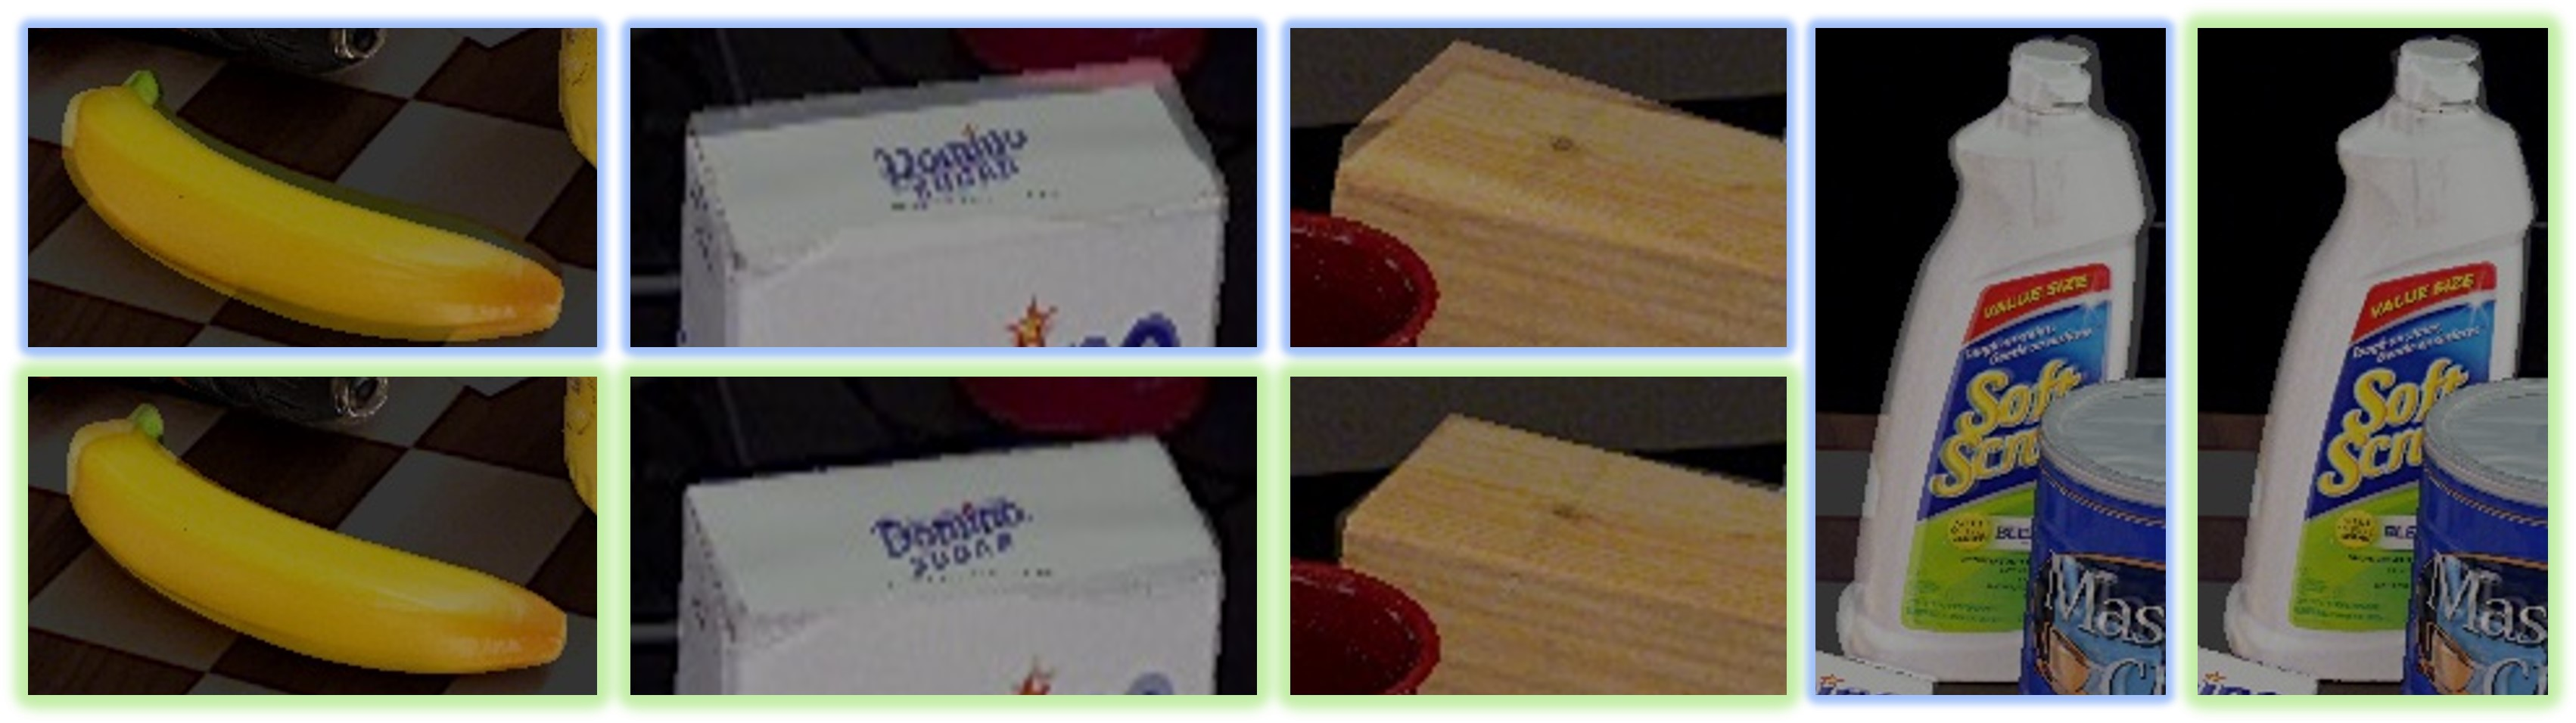
\includegraphics[width=0.97\textwidth]{figure/ca/detail_compare.jpg}}
    \caption{详细比较}
    \label{fig: detail_compare}
\end{figure*}

\textbf{轮廓对齐 } 对齐前后的CoI、$\mathbf{C}_\text{ren}$和$e_i$在\autoref{fig:optimization_vis}中可视化。左:RGB图像。中间和右:对齐前后的CoI、$\mathbf{C}_\text{ren}$和$e_i$。为了更好的可视化,$e_i$被稀疏绘制。文本的颜色与相应的视觉元素的颜色一致。

\textbf{失败案例 } 失败案例在\autoref{fig: failure_case}中可视化。最左列:RGB图像。中间列:SymNet结果。最右列:细化后的结果。大多数失败案例涉及严重遮挡的物体。几乎所有这些失败的主要原因是存在显著的初始值误差。没有发现优化导致结果显著恶化的例子。这突出了本文提出的细化方法的局限性,因为它对较大的误差没有影响。

\begin{figure}[t]
    \centering
    \begin{overpic}[width=0.70\textwidth]{figure/ca/optimization_vis.jpg}
        \put (35,4) {\textcolor{red}{$e = 2.69$}}
        \put (69,4) {\textcolor{red}{$e = 0.64$}}
        \put (39,25) {\textcolor{black}{CoI}}
        \put (73,25) {\textcolor{black}{CoI}}
        \put (52,18) {\textcolor{cyan}{$\mathbf{C}_\text{ren}$}}
        \put (85,18) {\textcolor{cyan}{$\mathbf{C}_\text{ren}$}}
    \end{overpic}
    \caption{轮廓对齐}
    \label{fig:optimization_vis}
\end{figure}

\begin{figure}[htbp]
\centerline{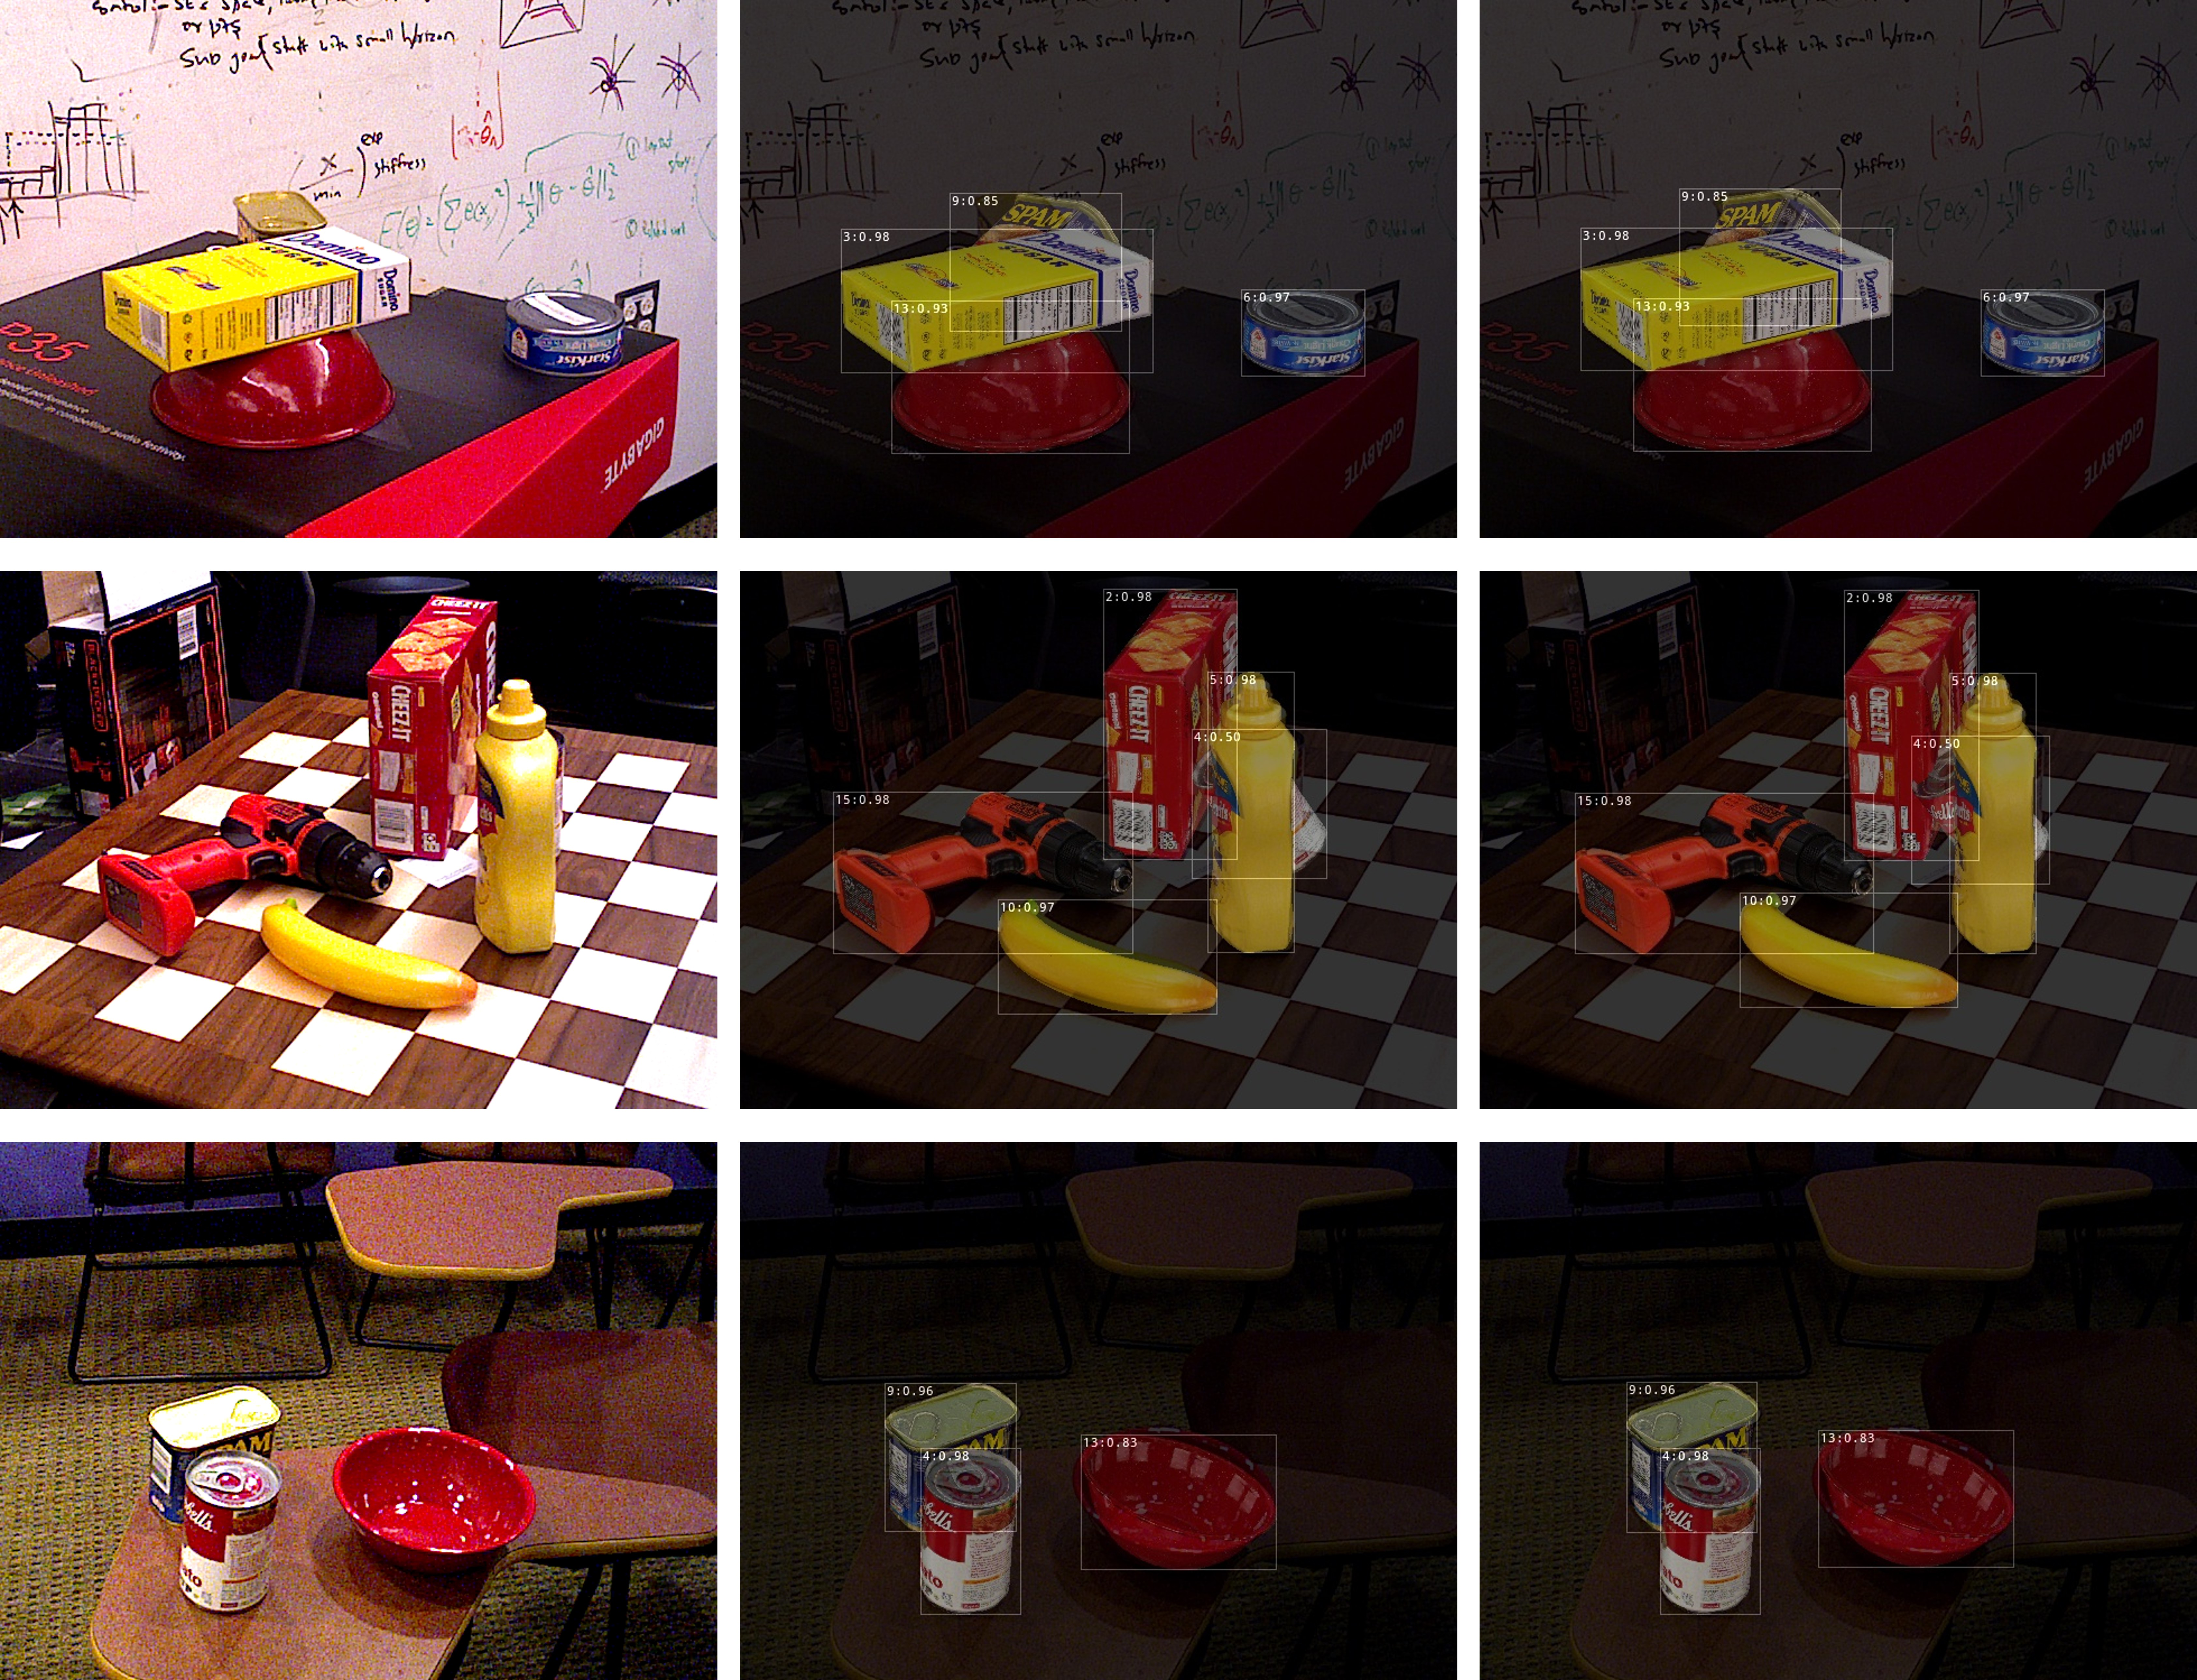
\includegraphics[width=0.70\textwidth]{figure/ca/failure_case.jpg}}
    \caption{失败案例 }
    \label{fig: failure_case}
\end{figure}
